
Parámetros del test: 
Cantidad de iteraciones por filtro-version 20.

\begin{figure}[h]
  \begin{center}
	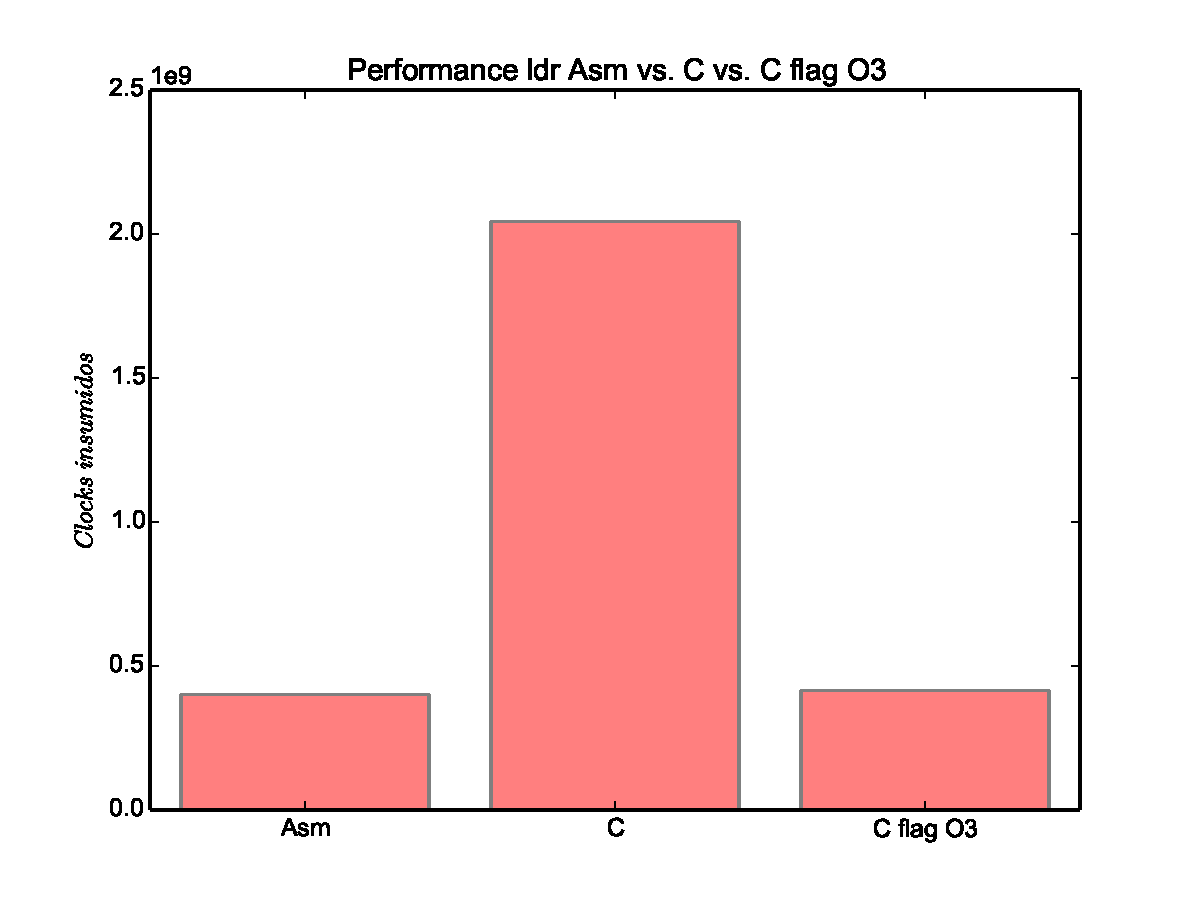
\includegraphics[scale=0.5]{ldr.pdf}
	%\caption{La última de Star Wars}
  \end{center}
\end{figure}

\begin{figure}[h]
  \begin{center}
	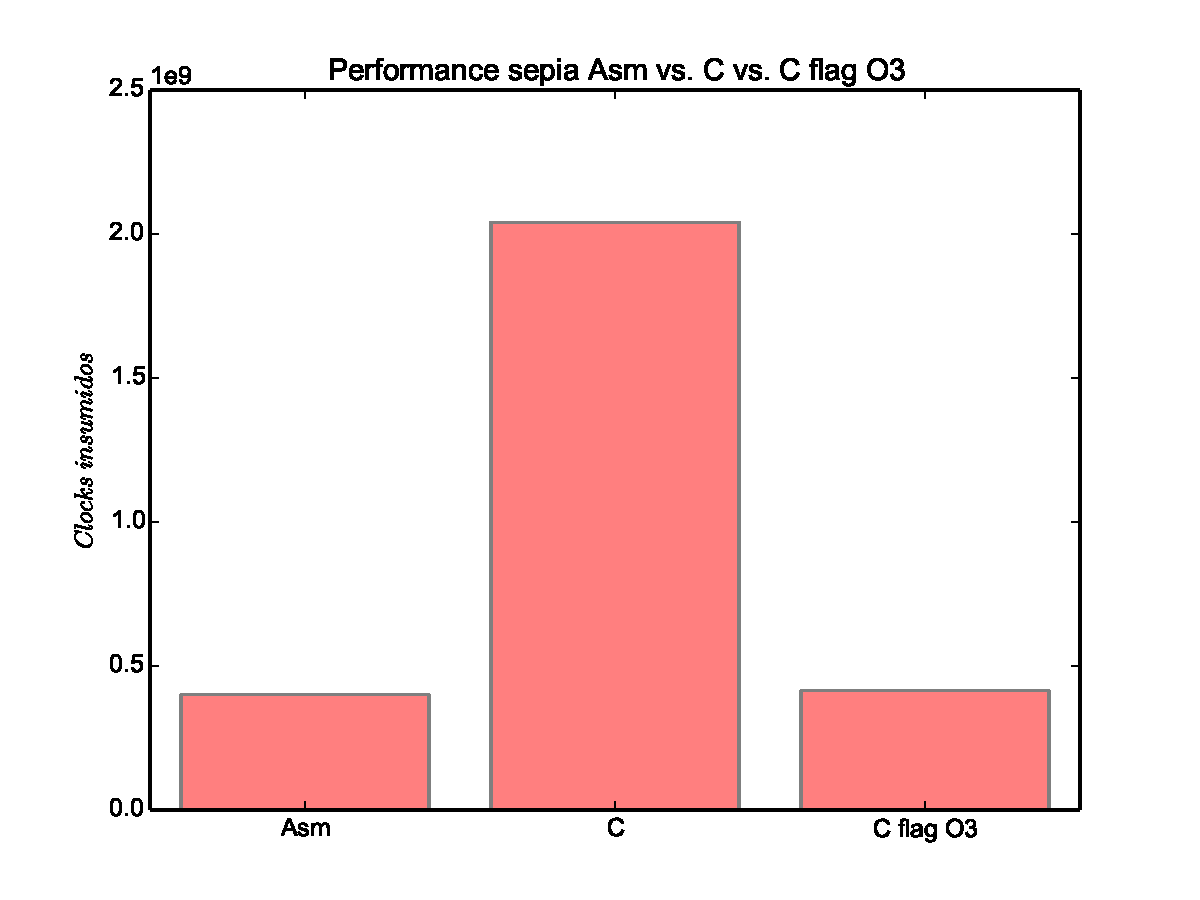
\includegraphics[scale=0.5]{sepia.pdf}
	%\caption{La última de Star Wars}
  \end{center}
\end{figure}

\newpage

\begin{figure}
  \begin{center}
	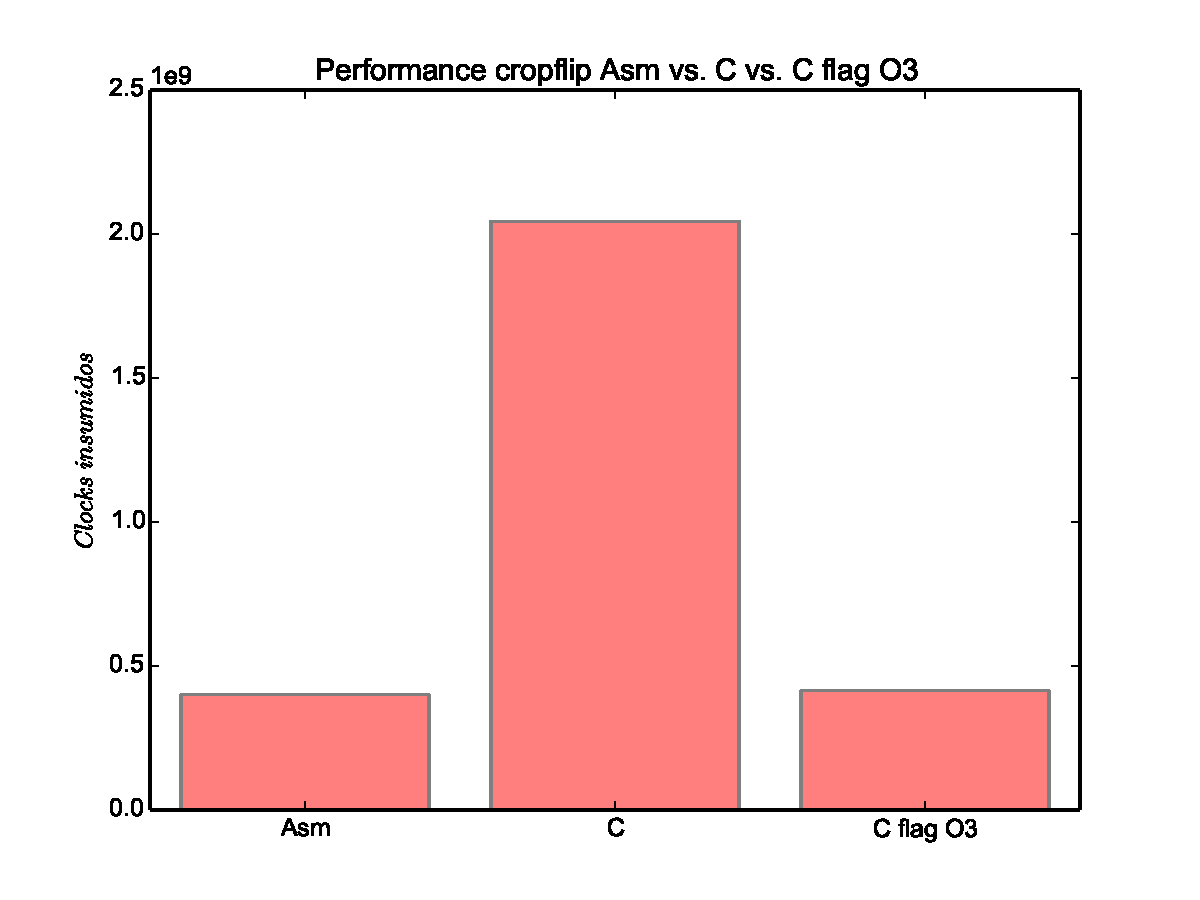
\includegraphics[scale=0.5]{cropflip.pdf}
	%\caption{La última de Star Wars}
  \end{center}
\end{figure}

Concluimos que los algoritmos escritos en $assembler$ son más rápidos quelos escritos en $C$. \\
Aunque podemos observar que en $C$ compilado con flag de optimizacion $O3$ llega a tener una performance muy similar.  \\

\newpage
